\chapter{Data Encryption in Linux Systems}
\label{chapter:enc-linux}

This chapter explains more detailed the concept of encryption and presents the handling of data encryption in traditional (non-Android) Linux systems.

\section{Encryption explained}
\label{sec:enc-explained}

%http://library.ahima.org/xpedio/groups/public/documents/ahima/bok1_048923.hcsp?dDocName=bok1_048923
Encryption is a mathematical transformation which scrambles data requiring protection (plaintext) into a form not easily understood by unauthorized entities (ciphertext). After being transformed into ciphertext, the plaintext appears random and does not reveal anything about the content of the original data.

Encryption is a reversible transformation. This reversal process is referred to as decryption. An encryption process has a corresponding decryption process, which is used to reverse the encrypted data (ciphertext) back to its original content (plaintext).

Each encryption and decryption function requires a cryptographic key. A cryptographic key is a string of binary digits used as an input to encryption and decryption functions.

\begin{figure}[h]
\centering
\begin{minipage}{0.45\textwidth}
\centering
  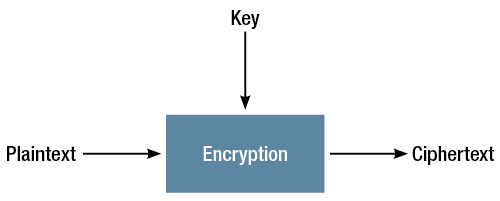
\includegraphics[width=.9\linewidth]{src/img/encrypt/plain2cipher.jpg}
  \caption{Encryption}
  \label{fig:encrypt-fig}
\end{minipage}\hfill
\begin{minipage}{0.45\textwidth}
\centering
  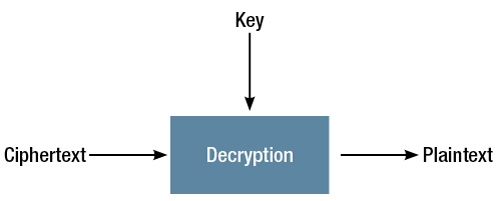
\includegraphics[width=.9\linewidth]{src/img/encrypt/cipher2plain.jpg}
  \caption{Decrpytion}
  \label{fig:decrypt-fig}
\end{minipage}
\end{figure}

For the purposes of disk encryption, each blockdevice (or individual file in the case of stacked filesystem encryption) is divided into sectors of equal length, for example 512 bytes (4,096 bits). The encryption/decryption then happens on a per-sector basis, so the n'th sector of the blockdevice/file on disk will store the encrypted version of the n'th sector of the original data.

Whenever the operating system or an application requests a certain fragment of data from the blockdevice/file, the whole sector (or sectors) that contains the data will be read from disk, decrypted on-the-fly, and temporarily stored in memory:

Similarly, on each write operation, all sectors that are affected must be re-encrypted complelety (while the rest of the sectors remain untouched).

In order to be able to de/encrypt data, the disk encryption system needs to know the unique secret key associated with it. Whenever the encrypted block device or folder in question is to be mounted, its corresponding key (called henceforth its \textit{master key}) must be supplied.

The following are some of the possible methods of storing and cryptographically securing a master key with a keyfile:
\begin{enumerate}
\item \textbf{Stored in a plaintext keyfile}

Simply storing the master key in a file (in readable form) is the simplest option. The file, called a \textit{keyfile}, can be placed on a removable device that is only connected to the computer when mounting the encrypted parts of the disk.

\item \textbf{Randomly generated on-the-fly for each session}

In some cases, e.g. when encrypting swap space or a /tmp partition, it is not necessary to keep a persistent master key at all. A new throwaway key can be randomly generated for each session, without requiring any user interaction. This means that once unmounted, all files written to the partition in question can never be decrypted again by anyone - which in those particular use-cases is perfectly fine.

\item \textbf{Stored in passphrase-protected form in a keyfile or on the disk itself}

The master key can be protected with a secret passphrase, which will need to be entered each time the encrypted block device or folder is mounted.
It is usually not used for de/encrypting the disk data directly, though. For example, in the case of stacked filesystem encryption, each file can be automatically assigned its own encryption key. Whenever the file is to be read/modified, this file key first needs to be decrypted using the main key, before it can itself be used to de/encrypt the file contents.

\end{enumerate}

\subsection{Benefits of disk encryption}
\label{sub-sec:benefits-enc}

Disk encryption is the process of storing data on disk in an encrypted form. The files only become available to the operating system and applications in readable form while the system is running and unlocked with the corresponding key.

Disk encryption methods aim to provide three distinct properties:
\begin{enumerate}
\item The data on the disk should remain confidential
\item Read and write operations should both be fast, regardless of where on the disk the data is stored
\item The overhead introduced by the encryption method should not be kept to a minimum (i.e., the amount of storage used for encrypted data should not be significantly larger than the size of plaintext)
\end{enumerate}

Disk encryption can prevent unauthorized viewing of the data when the computer or hard-disk is:
\begin{itemize}
\item located in a place to which non-trusted people might gain access while you are away
\item lost or stolen, as with laptops, netbooks or external storage devices
\item in the repair shop
\item discarded after its end-of-life
\end{itemize}

The system will still be vulnerable to:
\begin{itemize}
\item Attackers who can break into the system (e.g. over the Internet) while it is running and after the encrypted parts of the disk have already been unlocked and mounted.
\item Attackers who are able to gain physical access to the computer while it is running (even if you use a screenlocker), or very shortly after it was running, if they have the resources to perform a cold boot attack.
\item A government entity which may obtain your keys/passphrases using various techniques of coercion. It may be legal for law enforcement agencies to do so if they have suspicions that you might be hiding something of interest.
\end{itemize}

\subsection{Data Encryption vs System Encryption}
\label{sub-sec:de-vs-se}

\textbf{Data encryption} is defined as encrypting only the user's data itself (often located within the /home directory). While it is the simplest and least intrusive use of disk encryption, it has some significant drawbacks.
In modern computing systems, there are many background processes that may cache/store information about user data or parts of the data itself in non-encrypted areas of the hard drive, like:
\begin{itemize}
\item swap partitions
\item /tmp (temporary files created by user applications)
\item /var (log files and databases)
\end{itemize}


\textbf{System encryption} is the encryption of the operating system and user data, which helps to address some of the inadequacies of data encryption.

Benefits:
\begin{itemize}
\item prevents unauthorized physical access to operating system files
\item prevents unauthorized physical access to private data that may be cached by the system
\end{itemize}
Disadvantages:
\begin{itemize}
\item unlocking of the encrypted parts of the disk can no longer happen during or after user login; it must now happen at boot time
\end{itemize}
In practice, there is not always a clear line between data encryption and system encryption.

Finally, it is important that disk encryption be viewed as an adjunct to the existing security mechanisms of the operating system, while relying on other parts of the system to provide things like network security and user-based access control.

\subsection{Block Encryption vs Stacked File System Encryption}
\label{sub-sec:be-vs-sfse}

The two approaches to disk encryption are block-based and file-based. Block encryption means that the actual encryption process happens when the filesystem writes a block of data on the disk. Its advantages are simplicity and transparency. However, the method lacks granularity, i.e., treating each file differently. This is the type of encryption used in Android 3.0 and later.

A more in detail comparison of block-based encryption and file-based encryption is presented in the following table.\footnote{\url{http://ksouedu.com/doc/ecryptfs-utils/ecryptfs-faq.html\#compare}}

\renewcommand{\arraystretch}{1.8}
\begin{center}
\begin{table}[tp]
	\begin{tabularx}{\textwidth}{|| m{0.46\textwidth} || m{0.46\textwidth} ||}
		\hhline{|t:=:t:=:t|}
		\multicolumn{1}{||c||}{\textbf{Block Device Encryption}} & 
			\multicolumn{1}{c||}{\textbf{Stacked Filesystem Encryption}} \\ 
		\hhline{|:=::=:|}
		Simple in concept and implementation; just transform blocks as they pass through. & High level of design complexity; meticulous handling of internal filesystem primitives required. \\
		\hhline{|:=::=:|}
		Must allocate a block device to dedicate for the entire filesystem. & Stacks on top of existing mounted filesystems; requires no special on-disk storage allocation effort. \\
		\hhline{|:=::=:|}
		Everything in the filesystem incurs the cost of encryption and decryption, regardless of the confidentiality requirements for the data. & Selective encryption of the contents of only the sensitive files. \\
		\hhline{|:=::=:|}
		Fully protects the confidentiality of the directory structures, superblocks, file sizes, file permissions, and so forth. & Cannot keep all filesystem metadata confidential. Since stacked filesystems encrypt on a per-file basis, attackers will know the approximate file sizes, for instance. \\
		\hhline{|:=::=:|}
		Coarse granularity; only fixed per-mountpoint encryption policies are possible. & Fine granularity; flexible per-file encryption policies are possible. \\
		\hhline{|:=::=:|}		
		No notion of ``encrypted files.'' Individual files must be re-encrypted via a userspace application before written to backups, sent via email, etc. & Individual encrypted files can be accessed transparently by applications; no additional work needed on the part of applications before moving the files to another location. \\
		\hhline{|:=::=:|}
		Clients cannot use directly on networked filesystems; encryption must be set up and managed on the server, or the client must encase all of his files in a loopback mount, losing the per-file granularity from the perspective of other clients. & Clients can stack on locally mounted networked filesystems; individual files are sent to the server and stored in encrypted form. \\
		\hhline{|:=::=:|}
		Can protect databases that use their own dedicated block device. & Can only protect databases that write their tables to regular files in an existing filesystem. \\
		\hhline{|:=::=:|}
		Used to protect swap space. & Not designed to protect swap space; we recommend using block device encryption to protect swap space while using eCryptfs on the filesystem. \\
		\hhline{|:=::=:|}
		Possible to hide the fact that the partition is encrypted. & The fact that encrypted data exists on the device is obvious to an observer. \\
		\hhline{|:=::=:|}
		Filesystem-agnostic; any filesystem will work on an encrypted block device. & Can only be expected to work with existing filesystems that are upstream in the official Linux kernel. \\
		\hhline{|b:=:b:=:b|}
	\end{tabularx}
	\caption{Block Device Encryption vs Stacked Filesystem Encryption}
\end{table}
\end{center}
\newpage

\section{eCryptfs}
\label{sec:de-ecryptfs}

As mentioned before, eCryptfs is a stacked file system which manages data encryption. Now, details about it and the advantages and disadvantages is brings will be presented.

Originally authored by Michael Halcrow and the IBM Linux Technology Center, eCryptfs is derived from Erez Zadok's Cryptfs, and the FiST framework for stacked filesystems. eCryptfs extended Cryptfs to provide advanced key management and policy features.\footnote{\url{http://uni-smr.ac.ru/archive/linux/linuxsymposium_procv1.pdf\#page=209}}

It has already been mentioned that eCryptfs uses a randomly generated File Encyption Key(FEK) for each file and that this key is also encrypted. Also noteworthy is that the FEK in its encrypted form is actually stored together with the encrypted file. This adds the posibility of transfering a file while encrypted with the ability to gain access with the proper credentials.

\subsection{Architecture}
\label{sub-sec:arch-ecryptfs}

eCryptfs is implemented as a kernel module augmented with various userspace utilities for performing key management functions.

\fig[scale=0.24]{src/img/ecryptfs/arch.png}{img:ecryptfs-arch}{eCryptfs Architecture}

The kernel module encrypts the file contents using the kernel cryptographic API. A keystore component extracts the header information from individual files and forwards this data to a callout application. The callout application evaluates the header information against the target policy and performs various operations, such as prompting the user for a passphrase or decrypting a session key with a private key.

Key management is done in userspace for two main reasons. The first is to reduce the complexity of the code running in kernelspace. The second is due to the fact that management operation are only required when opening/closing a file. Since these operations are relatively infrequent, the overhead does not constitute an issue.

Below is the flow of an open operation on a system using ecryptfs.

\begin{figure}[h!]
\centering
    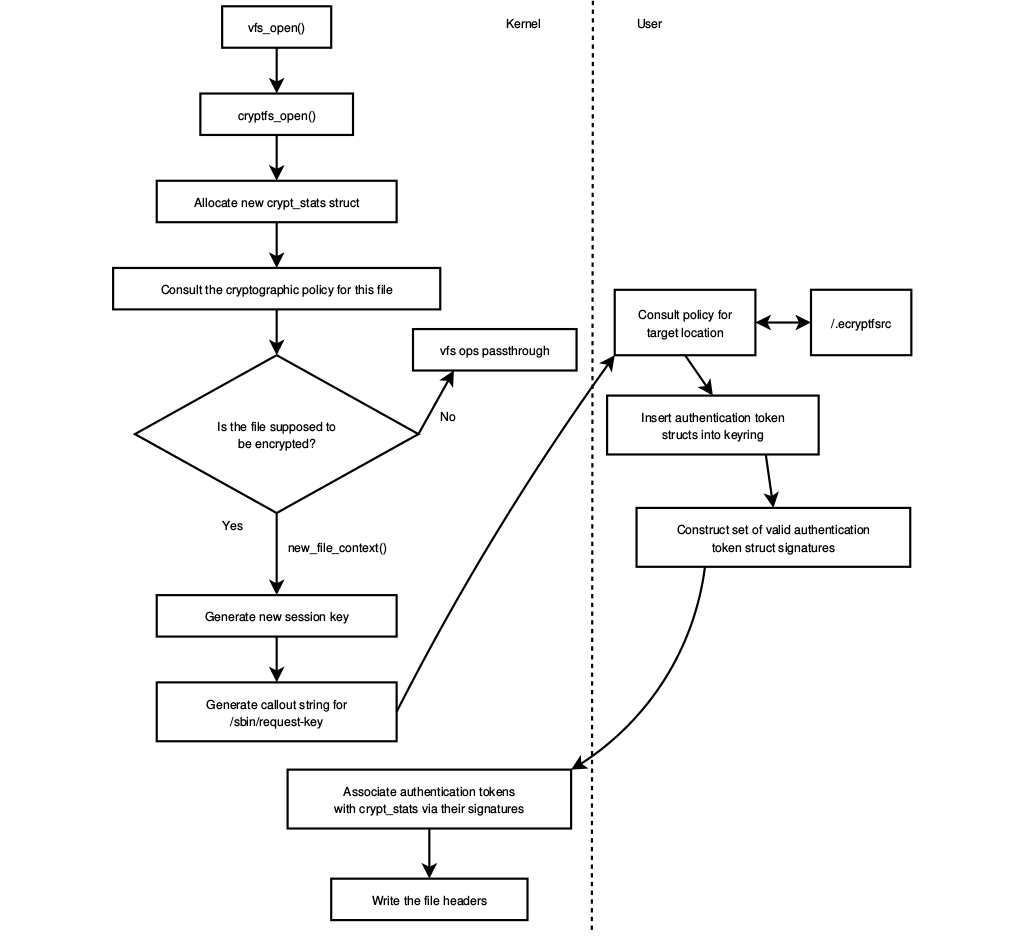
\includegraphics[width=0.9\textwidth]{src/img/ecryptfs/newfile.png}
\caption{eCryptfs Open File Process}
\end{figure}

\subsection{Cryptographic Operations}
\label{sub-sec:crypt-ops-ecryptfs}

Most of the data encryption is done in the kernel module, and hence eCryptfs makes use of the kernel cryptographic API to perform the encryption and the decryption operations. One of the primary motivators in implementing eCryptfs in the kernel is to avoid the overhead of context switches between userspace and kernel space, which is frequent when dealing with pages in file I/O. Any symmetric ciphers supported by the Linux kernel can be used as the bulk data ciphers for the eCryptfs files.

The underlying file format for eCryptfs is based on the OpenPGP format described in RFC2440\footnote{\url{ftp://ftp.rfc-editor.org/in-notes/rfc2440.txt}}

\begin{figure}[h!]
\centering
    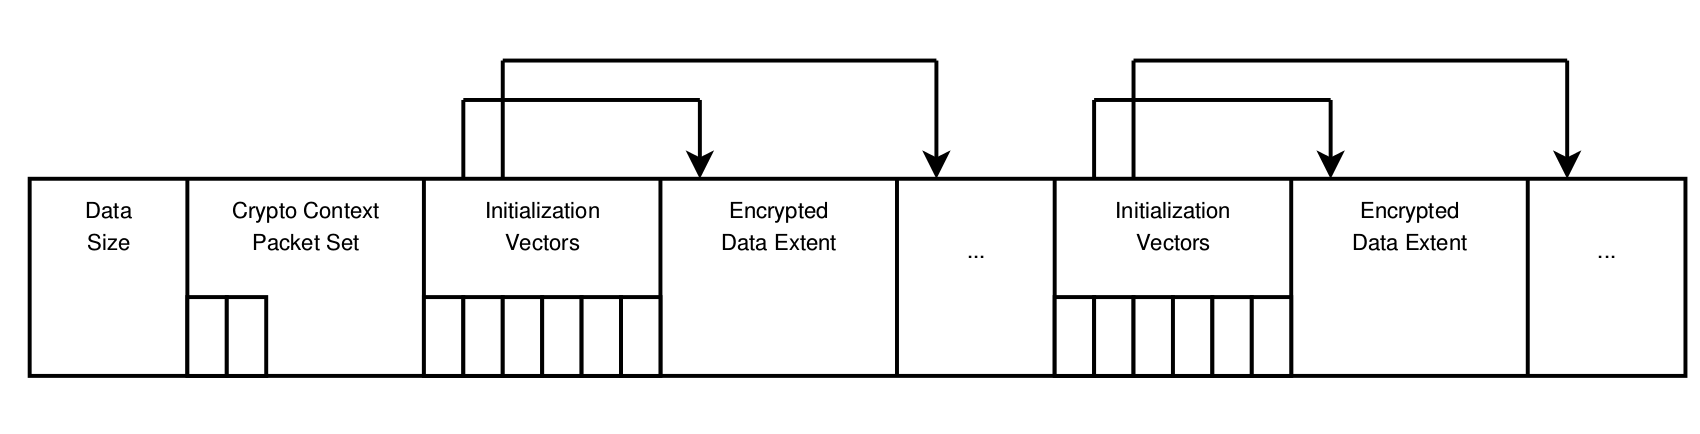
\includegraphics[width=0.92\textwidth]{src/img/ecryptfs/fileformat.png}
\caption{eCryptfs File Format}
\end{figure}

An aspect where eCryptfs deviates from the standard is the introduction of \textit{data extents}. This is done in order to accommodate random access while maintaining performance. The OpenPGP standard assumes that the encryption and decryption is done as an atomic operation over the entire data contents of the file; there is no concept of a partially encrypted or decrypted file. The data is encrypted using what is known as a chained block cipher(CBC\abbrev{CBC}{Chained Block Cipher}). This means that each block of plaintext, with the exception of the first, is combined with the previous block ciphertext through a XOR operation before being encrpyted. Evidently, the same process must be followed when decrypting. Thus, reading a byte from a file requires decrypting all leading bytes. Conversely, writing a byte incurs encrypting all trailing bytes from that file. For large files, reading a byte towards the end of the file or writing a byte at the beginning of it would be inefficient.

Using extents, each part of a file is encrypted separately; reading or writing a byte requires operations only on the extent containing the respective byte. The extents span the page size (as specified for each kernel build). An extent containing initialization vectors(IV\abbrev{IV}{Initialization Vector}) precedes a group of extents which used the respective IV's (each extent has an unique IV). These initialization vectors are used to XOR the first block of data when encrypting/decrypting.

Another challenge is treating \textit{sparse files}. According to UNIX semantics, a file becomes sparse when an application seeks past the end of it. These results in regions where no data is written, also known as \textit{holes}. The file system normally uses special markers for these regions and sets the filesize in accordance. Thus, less space on the disk is used to store the file. When reading from these regions, the file system simply fills in with zero's.

Although eCryptfs could use markers, e.g. IV's consisting of all zero's, to implement a similar behaviour, this may constitute a breach in security, since it becomes readily apparent to a potential attacker which regions are sparse.
Therefore, eCryptfs prefers to relegate how to treat sparse files to something policy decides.

\subsection{Key Management}
\label{sub-sec:keys-ecryptfs}

eCryptfs aims to operate transparently. The fact that files are encrypted should not be a concern to the user.

Every file receives a randomly generated session key, which is used in the bulk data encryption of the file contents. This session key is stored in the cryptographic metadata for the file, which is in turn cached in the user’s session keyring. When an application closes a newly created file, eCryptfs encrypts the session key once for each authentication token associated with that file, as dictated by policy, then writes these encrypted session keys into packets in the header of the underlying file.
When an application later opens the file, eCryptfs reads in the encrypted session keys and chains them off of the cryptographic metadata for the file. eCryptfs looks through the user’s authentication tokens to attempt to find a match with the encrypted session keys; it uses the first one found to decrypt the session key. In the event that no authentication tokens in the user’s session keyring can decrypt any of the encrypted session key packets, eCryptfs falls back on policy. This policy can dictate actions such as querying PKI modules for the existence of private keys or prompting the user for a passphrase.

Passphrase authentication tokens in eCryptfs exist in three forms: non-passphrased, saltless, and salted. In order to address the threat of passphrase dictionary attacks, eCryptfs utilizes the method whereby a salt value is concatenated with a passphrase to generate a passphrase identifier. The concatenated value is iteratively hashed (65,537 times by default) to generate the identifying signature for the salted authentication token.

The key callout application is the primary contact between the eCryptfs kernel module and the userspace key management code. This callout application parses policy information from the target, which it interprets in relation to the header information in each file. It may then make calls through the PKI API in order to satisfy pending public key requests, or it may go searching for a salted passphrase with a particular signature. The eCryptfs daemon listens to a socket (for which the location is written to the user’s session keyring). Whenever policy calls for the user to be prompted for a passphrase, the callout application can retrieve the socket’s location and use it to request the daemon to prompt the user; the daemon then returns the user’s passphrase to the callout application.

\subsection{Encrypting a Directory Using eCryptfs}
\label{sub-sec:encrypt-dir-ecryptfs}

This is an example of how to encrypt a user directory. It relies on the \textit{ecryptfs-utils} package being installed. Although the operations can be performed manually, for the purpose of this example there is no need to go into such amount of detail. More details on the Arch Linux page on eCryptfs.\footnote{\url{https://wiki.archlinux.org/index.php/ECryptfs}}

The name \texttt{secret} will be used for the created directory.

Firt step is to create the required directories:
\begin{lstlisting}[numbers=none]
$ mkdir ~/.secret ~/secret ~/.ecryptfs
$ touch ~/.ecryptfs/secret.conf ~/.ecryptfs/secret.sig
\end{lstlisting}

The encrypted data will be stored in the \texttt{\textasciitilde/.secret} directory.
\texttt{\textasciitilde/secret} is the location where the \texttt{\textasciitilde/.secret} will be mounted as an eCryptfs file system.

Next, the full paths must be added to \texttt{\textasciitilde/.ecryptfs/secret.conf}. They will be used later to mount/unmount data.
\begin{lstlisting}[numbers=none]
$ echo "/home/$USER/.secret /home/$USER/secret ecryptfs" > ~/.ecryptfs/secret.conf
\end{lstlisting}
Note that \texttt{\$USER} should be expanded by the shell to the current username.

A mount passphrase must be added to the keyring:
\begin{lstlisting}[numbers=none]
$ ecryptfs-add-passphrase
Passphrase: 
Inserted auth tok with sig [78c6f0645fe62da0] into the user session keyring
\end{lstlisting}

The ouput signature is added to \texttt{\textasciitilde/.ecryptfs/secret.sig}
\begin{lstlisting}[numbers=none]
$ echo 78c6f0645fe62da0 > ~/.ecryptfs/secret.sig
\end{lstlisting}

Optionally, a passphrase for filename encryption can be appended to the same file
\begin{lstlisting}[numbers=none]
$ ecryptfs-add-passphrase
Passphrase: 
Inserted auth tok with sig [326a6d3e2a5d444a] into the user session keyring
 $ echo 326a6d3e2a5d444a >> ~/.ecryptfs/secret.sig
\end{lstlisting}

To mount \texttt{\textasciitilde/.secret} on \texttt{\textasciitilde/secret}:
\begin{lstlisting}[numbers=none]
$ mount.ecryptfs_private secret
\end{lstlisting}
The mount options are automatically generated using the information stored in \texttt{secret.conf} and \texttt{secret.sig}.

Similarly, to unmount:
\begin{lstlisting}[numbers=none]
$ umount.ecryptfs_private secret
\end{lstlisting}
